%%%%%%%%%%%%%%%%%%%%%%%%%%%%%
%% Styles, packages and new commands
\input{../../Main/ML_Main.tex}
%%%%%%%%%%%%%%%%%%%%%%%%%%%%%
%% Edit the title page
\title{Machine Learning}
\subtitle{Module 3.3 - Models: Neural Networks}
\author[MOB]{Marc-Olivier Boldi}
\institute[HEC MSc Mgt BA]{Master in Management, Business Analytics, HEC UNIL}
\date[Spring 2024]{Spring 2024}
%%%%%%%%%%%%%%%%%%%%%%%%%%%%%
%%%%%%%%%%%%%%%%%%%%%%%%%%%%%
%%%%%%%%%%%%%%%%%%%%%%%%%%%%%
%%%%%%%%%%%%%%%%%%%%%%%%%%%%%
\begin{document}
	\begin{frame}
	\titlepage
	\end{frame}
%%%%%%%%%%%%%%%%%%%%%%%%%%%%%
\section{Concept and prediction formula}
%%%%%%%%%%%%%%%%%%%%%%%%%%%%%
\begin{frame}
\frametitle{Artificial Neural Network}
{\bf Artificial Neural networks} are models used for classification and for regression based on combining several predictions of small nodes. To illustrate the method we are applying it on the {\tt iris} data set, without splitting between training and test sets. \\ 
\vspace{0.3cm}
{\bf Example}: {\tt iris} data with 3 possible classes, {\tt Setosa}, {\tt Virginica}, and {\tt Versicolor} to be predicted from 4 features {\tt Sepal.Length} $(x_1)$, {\tt Sepal.Width} $(x_2)$, {\tt Petal.Length} $(x_3)$, and {\tt Petal.Width} $(x_4)$. 
\end{frame}
%%%%%%%%%%%%%%%%%%%%%%%%%%%%%
\begin{frame}
\frametitle{Example}
A neural network looks like this
\begin{columns}
\begin{column}{0.6\linewidth}
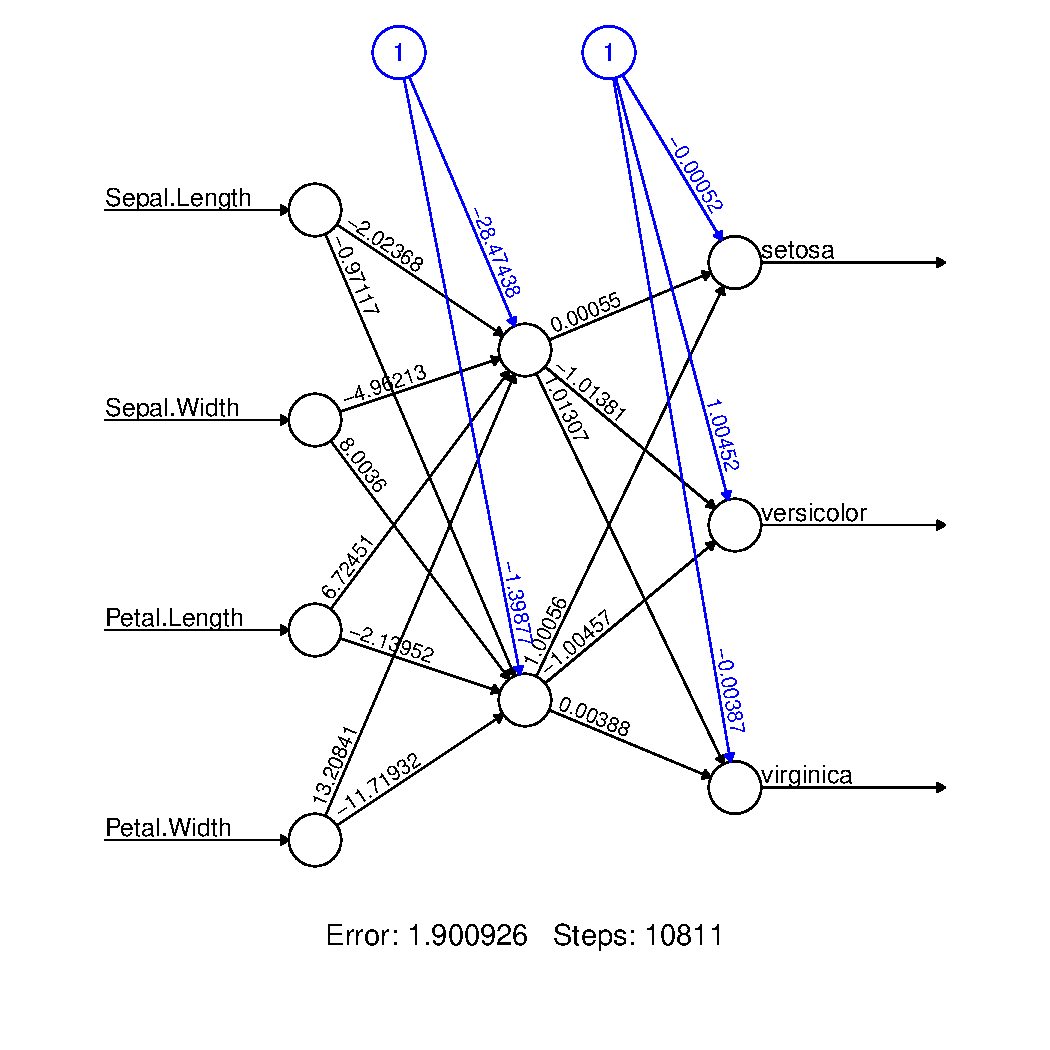
\includegraphics[width=8cm]{../../Graphs/NN_Iris.pdf}
\end{column}
\begin{column}{0.4\linewidth}
\begin{itemize}
\item 4 input {\bf nodes} (circles) 
\item Arrows with {\bf weights}.
\item One middle {\bf layer} made of 2 $(+1)$ nodes.
\item 3 output nodes: one for each class (species).
\end{itemize}
\end{column}
\end{columns}
\end{frame}
%%%%%%%%%%%%%%%%%%%%%%%%%%%%%
\begin{frame}
\frametitle{Parameters}
In the context of NN, people use the term {\bf weights} to talk about the parameters of the model, $\theta$.\\
\vspace{0.3cm}
E.g., on the middle layer, coefficients are associated to the arrows:
\begin{itemize}
\item One constant term (node "1") called the {\bf bias}: 
$$
\theta_{11}^{(0)}=-28.5
$$
\item One coefficient per arrows: 
$$
\theta_{11}^{(1)}=-2.02, \ldots, \theta_{11}^{(4)}=13.21.
$$
\end{itemize}
\end{frame}
%%%%%%%%%%%%%%%%%%%%%%%%%%%%%
\begin{frame}
\frametitle{Node value}
Arrows interring a node indicate a weighted sum of at the previous node values. E.g., consider the top node of the middle layer:
\begin{eqnarray*}
\eta_{11} &=& \theta_{11}^{(0)} + \theta_{11}^{(1)} x_1 + \cdots + \theta_{11}^{(4)} x_4\\
&=& -28.5 -2.0 x_1 + \cdots + 13.2 x_4
\end{eqnarray*}
Then the {\bf sigmoid function}\footnote{See logistic regression.}. function is applied to obtain the value at the top node of the middle layer:
\begin{eqnarray*}
Z_{11} &=& \sigma(\eta_{11}) = \frac{e^{\eta_{11}}}{1+e^{\eta_{11}}}
\end{eqnarray*}
This is repeated at the second middle node:
\begin{eqnarray*}
\eta_{12} &=& \theta_{12}^{(0)} + \theta_{12}^{(1)} x_1 + \cdots + \theta_{12}^{(4)} x_4\\
&=& -1.4 -1.0 x_1 + \cdots - 11.7 x_4\\
Z_{12} &=& \sigma(\eta_{12}) = \frac{e^{\eta_{12}}}{1+e^{\eta_{12}}}
\end{eqnarray*}
\end{frame}
%%%%%%%%%%%%%%%%%%%%%%%%%%%%%
\begin{frame}
\frametitle{The output}
The $Z$ values are now passed to the outcome nodes. E.g., at {\tt setosa}:
\begin{eqnarray*}
\eta_{12} &=& \theta_{12}^{(0)} + \theta_{12}^{(1)} Z_{11} + \theta_{12}^{(1)} Z_{21} \\
 &=& 0.0 + 0.0 Z_{11} - 1.0 Z_{21} \\
\end{eqnarray*}
The calculation is repeated for each node giving $\eta_{12}, \eta_{22}, \eta_{32}$. Then, the value of the node is obtained applying the {\bf soft-max} function:
\begin{eqnarray*}
Z_{12} &=& \frac{e^{\eta_{12}}}{e^{\eta_{12}}+e^{\eta_{22}}+e^{\eta_{32}}},\\
Z_{22} &=& \frac{e^{\eta_{22}}}{e^{\eta_{12}}+e^{\eta_{22}}+e^{\eta_{32}}},\\
Z_{32} &=& \frac{e^{\eta_{32}}}{e^{\eta_{12}}+e^{\eta_{22}}+e^{\eta_{32}}}.
\end{eqnarray*}
\end{frame}
%%%%%%%%%%%%%%%%%%%%%%%%%%%%%
\begin{frame}
\frametitle{The prediction formula}
The values at the output are the probabilities of each class predicted for the input $x$:
$$
p_c(x;\theta) = Z_{c2}, \quad c=1,2,3.
$$
Indeed, the soft-max guaranties that
$$
0 < Z_{c2} < 1, \quad Z_{12}+Z_{22}+Z_{32} = 1.
$$
The prediction for $x$ is the class with maximum probability:
$$
f(x;\theta) = \arg \max_{c=1,\ldots,C} p_c(x;\theta).
$$
\end{frame}
%%%%%%%%%%%%%%%%%%%%%%%%%%%%%
\begin{frame}
\frametitle{The regression case}
For the regression, the main difference is that the output layer is made of just one node whose value is the final prediction. In the example, 
$$
f(x;\theta) = \theta_{12}^{(0)} + \theta_{12}^{(1)} Z_{11} + \theta_{12}^{(1)} Z_{21}
$$
\end{frame}
%%%%%%%%%%%%%%%%%%%%%%%%%%%%%
\section{Neural network design}
%%%%%%%%%%%%%%%%%%%%%%%%%%%%%
\begin{frame}
\frametitle{Number of nodes and layers}
Building NN is kind of an art. Two important parameters are
\begin{itemize}
\item The number of middle layers called {\bf hidden} layers,
\item For each hidden layer, the number of nodes.
\end{itemize}
There is no general rule for this choices. One has to try and see if the quality follows.\\
\vspace{0.3cm} 
Empirical rules are
\begin{itemize}
\item Hidden layers with more nodes help creating new features (new dimensions).
\item Hidden layers with less nodes help combining the previous features to create strong features (dimension reduction).
\end{itemize}
\end{frame}
%%%%%%%%%%%%%%%%%%%%%%%%%%%%%
\begin{frame}
\frametitle{Activation functions}
In the example, the sigmoid function was applied at each hidden layer node. This is not the only available choice: other functions can be used. These function are called {\bf activation} functions.\\
\vspace{0.3cm}
For the hidden layers, usual choices are
\begin{itemize}
\item (so-called) {\bf Linear}; meaning no function (identity).
$$
g(x) = x
$$
\item Rectified Linear Activation {\bf ReLu}
$$
g(x) = \max(0,x)
$$
\item {\bf Sigmoid}
$$
g(x) = \frac{e^x}{1+e^x} = \frac{1}{1+e^{-x}}
$$
\end{itemize}
\end{frame}
%%%%%%%%%%%%%%%%%%%%%%%%%%%%%
\begin{frame}
\frametitle{Activation functions}
\begin{center}
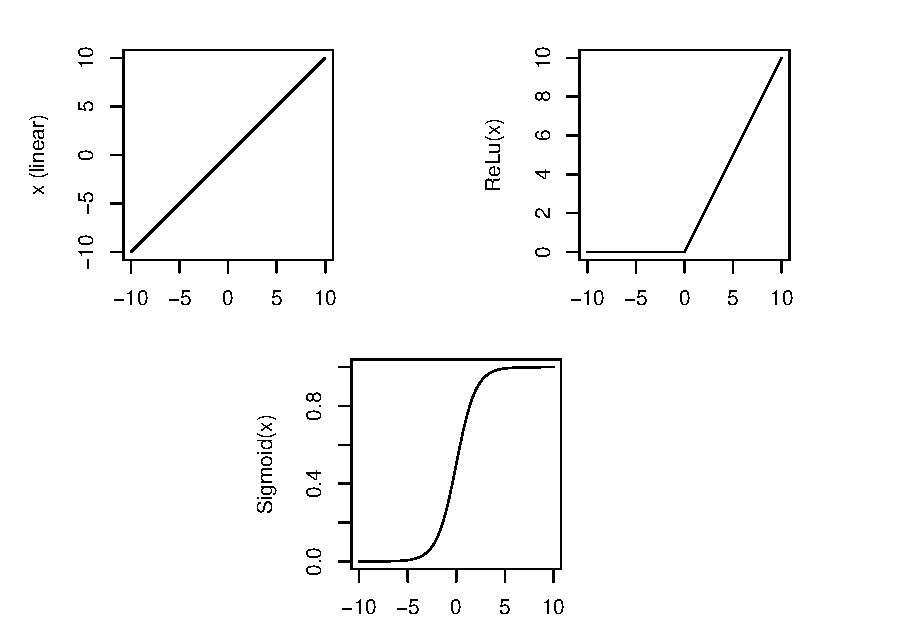
\includegraphics[width=10cm]{../../Graphs/Activation_graphs.pdf}
\end{center}
\end{frame}
%%%%%%%%%%%%%%%%%%%%%%%%%%%%%
\begin{frame}
\frametitle{Activation functions}
For the output layer, choices are
\begin{itemize}
\item Classification: {\bf softmax}
$$
g(x_c) = \frac{e^{x_c}}{\sum_{j=1}^C e^{x_j}}.
$$
\item Regression: same as hidden layers.
\end{itemize}
\end{frame}
%%%%%%%%%%%%%%%%%%%%%%%%%%%%%
\begin{frame}
\frametitle{Activation functions}
There is no one good way to do it, but there are plenty of errors that can be avoided:
\begin{itemize}
\item {\bf Use non-linearity}: if only the linear activation function is used in the hidden layer then the NN is a simple linear model. In particular,
\begin{itemize}
\item For regression: if the output layer has a linear activation then the NN is equivalent to a linear regression.
\item For binary classification: if the output layer has a sigmoid activation then the NN is equivalent to a logistic regression.
\end{itemize}
\item Watch the {\bf range of the output}. E.g., if $y$ is positive, then using a ReLu activation function close to the output may be good, whereas using a sigmoid on the output layer will prevent the NN to predict values larger than 1.
\item {\bf Mix activation functions} along the hidden layers: helps too learn non-linearities.
\end{itemize}
\end{frame}
%%%%%%%%%%%%%%%%%%%%%%%%%%%%%
\section{Loss functions}
%%%%%%%%%%%%%%%%%%%%%%%%%%%%%
\begin{frame}
\frametitle{Loss functions}
The most common loss functions are
\begin{itemize}
\item For regression, the MSE
$$
\bar{\cal L}(\theta) = \frac{1}{n} \sum_{i=1}^n \{y_i - f(x_i;\theta)\}^2.
$$
\item For classification, the cross-entropy
$$
\bar{\cal L}(\theta) = -\sum_{i=1}^n \sum_{c=1}^C 1_{\{y_i=c\}} \log p_c(x_i;\theta).
$$
\end{itemize}
Here, $\theta$ denotes all the NN parameters (weights). 
\end{frame}
%%%%%%%%%%%%%%%%%%%%%%%%%%%%%
\section{Training algorithm}
%%%%%%%%%%%%%%%%%%%%%%%%%%%%%
\begin{frame}
\frametitle{Gradient Descent}
The training is done by minimizing $\bar{\cal L}(\theta)$, which is an intensive computation.\\ 
\vspace{0.3cm}
The most used algorithm is the {\bf gradient descent}. 
\begin{itemize}
\item Start at a random set of weights $\theta$,
\item Update the weights using a descent direction (i.e., a direction guaranteeing a diminution of the loss), usually the negative gradient 
$$
\theta \leftarrow \theta - \eta \nabla \bar{\cal L}(\theta),
$$ 
\item Iterate until convergence.
\end{itemize}
Above, $\eta$ controls the learning rate. Its choice is crucial. It varies from iterations and can be a vector, i.e., one learning rate per weight (AdaGrad, RMSProp, Adam). 
\end{frame}
%%%%%%%%%%%%%%%%%%%%%%%%%%%%%
\begin{frame}
\frametitle{Backpropagation}
The computation of the gradient $\nabla \bar{\cal L}(\theta)$ can be very heavy on a NN.\\ 
\vspace{0.3cm}
{\bf Backpropagation} is a method exploiting the iterative structure of the network to compute this gradient. 
\end{frame}
%%%%%%%%%%%%%%%%%%%%%%%%%%%%%
\begin{frame}
\frametitle{Stochastic Gradient Descent}
If $n$ is large (lots of instances) 
$$
\nabla \bar{\cal L}(\theta)=\sum_{i=1}^n \nabla \bar{\cal L}_i(\theta)
$$ 
is heavy to compute. It can be approximated by a partial sum over a random subset of instances $S\subseteq \{1,\ldots,n\}$ : 
$$
\nabla \bar{\cal L}(\theta)=\sum_{i=1}^n \nabla \bar{\cal L}_i(\theta) \approx \sum_{i \in S} \nabla \bar{\cal L}_i(\theta)
$$ 
This is a called {\bf stochastic gradient descent} (SDG). 
\end{frame}
%%%%%%%%%%%%%%%%%%%%%%%%%%%%%
\begin{frame}
\frametitle{SDG: batches and epochs}
For SGD, the practice is to
\begin{itemize}
\item Split the set $\{1,\ldots,n\}$ randomly into $m$ {\bf batches} of the same size, $S_1,\ldots,m$,
\item Apply the gradient descent update step sequentially along the batches (in a random order). 
\item One pass through all the $m$ batches is called an {\bf epoch}.
\end{itemize}
The choice of the size of the batch is a compromise between computation time and the quality of the gradient approximation:
\begin{itemize}
\item A large batch size (at the limit $n$) makes the gradient heavy to compute but more accurate ($S\approx \{1,\ldots,n\}$). Each epoch has few iterations but each iteration is long. 
\item A small batch size makes the gradient fast to compute ($S$ is small) but approximate. Each epoch has a lot of short iterations.
\end{itemize}
\end{frame}
%%%%%%%%%%%%%%%%%%%%%%%%%%%%%
\section{Interpretation}
%%%%%%%%%%%%%%%%%%%%%%%%%%%%%
\begin{frame}
\frametitle{Interpretation}
NN are not interpretable. They are large model combining variables along several non-linear activation function layers. Specific methods can be used (see later in the course).
\end{frame}
%%%%%%%%%%%%%%%%%%%%%%%%%%%%%
\section{Model simplification}
%%%%%%%%%%%%%%%%%%%%%%%%%%%%%
\begin{frame}
\frametitle{Model complexity}
By construction NN are complex models: they have a lot of weights. E.g., even a small model with $10$ features, $2$ hidden layers with $(16,8)$ nodes, and 3 classes has 
$$
(10+1)\times 16 + (16+1)\times 8 + (8+1)\times 3 = 339
$$
weights. \\
\vspace{0.3cm}
With such a large number of parameters, the model is at risk of overfitting the training set by learning too much. One can regularize the model in a similar way to linear and logistic regressions.
\end{frame}
%%%%%%%%%%%%%%%%%%%%%%%%%%%%%
\begin{frame}
\frametitle{Regularization}
The idea is to use $L_1$ and/or $L_2$ penalties on the loss during the training
$$
\bar{\cal L}(\theta) + \lambda_1 \sum_{j} |\theta_j| + \lambda_2 \sum_{j} \theta_j^2.
$$ 
Again there is no simple way to set the penalty parameters $\lambda_1$ and $\lambda_2$. Note that it is possible to have different penalty parameters in different layers.\\
\vspace{0.3cm}
Unlike regression and trees, and like SVM, this regularization can help to avoid overfitting but cannot be interpreted easily. 
\end{frame}
%%%%%%%%%%%%%%%%%%%%%%%%%%%%%
\end{document}
%%%%%%%%%%%%%%%%%%%%%%%%%%%%%


%%%%%%%%%%%%%%%%%%%%%%%%%%%%%
\begin{frame}[fragile]
\frametitle{Example}
In the iris example, for flower 1, with features\\
\scriptsize
\begin{verbatim}
     Sepal.Length Sepal.Width Petal.Length Petal.Width
[1,]          5.1         3.5          1.4         0.2
\end{verbatim}
\normalsize
the values at the middle node are\\
\scriptsize
\begin{verbatim}
$`neurons`[[2]]                                                                         $
     [,1]         [,2]         [,3]
[1,]    1 6.994358e-20 9.999999e-01
\end{verbatim}
\normalsize
and the values ($T_c$) are\\ 
\scriptsize
\begin{verbatim}
$net.result                                                                            $
                [,1]          [,2]          [,3]
[1,]  1.000039e+00 -4.757805e-05  3.265727e-06
\end{verbatim}
\normalsize
The prediction is thus {\tt se}. 
\end{frame}
%%%%%%%%%%%%%%%%%%%%%%%%%%%%%
\begin{frame}
\frametitle{Several layers}
It is possible to extend the number of layers in the system like in the example below:
\begin{center}
\includegraphics[width=7cm]{../../Graphs/NN_Iris_2L.pdf}
\end{center}
\end{frame}
%%%%%%%%%%%%%%%%%%%%%%%%%%%%%
\begin{frame}
\frametitle{Several layers}
A NN contains lots of coefficients. For example, with 4 features, 2 middle layers, with respectively 2 and 3 nodes, and 3 classes, there are a total number of coefficients:
$$
(4+1)\times 2 + (2+1)\times 3 + (3+1) \times 3 = 10+9+12 = 31
$$
In general, with $p$ features, $K$ middle layers and $C$ output, the total number of parameters is
$$
(p+1)\times n_1 + \sum_{k=2}^K (n_{k-1}+1) \times n_k + (n_K+1)\times C,
$$
where $n_k$ is the number of nodes in layer $k$. This number is growing very fast with the number of layers and of nodes.\\
\vspace{0.2cm} 
Therefore, there are lots of coefficients to estimate. These are often called {\bf weights}.
\end{frame}
%%%%%%%%%%%%%%%%%%%%%%%%%%%%%
\begin{frame}
\frametitle{Estimation}
Then the following quantity is called the cross-entropy:
$$
CE = - \sum_{i=1}^n \sum_{c=1}^C y_{ic}\log f_c(x_i).
$$
It is an impurity measure that is minimized on the training set to find the weights.
Above we have
\begin{itemize}
\item $n$ the number of instances $i$, 
\item $C$ the number of classes $c$,
\item The outcome $y_i$ is coded\footnote{The $1$ is in position $c$ when the outcome is class $c$} 
$$
y_{i}=(0, 0, \ldots, 1, 0, \ldots, 0)
$$ 
Correspondingly $y_{ic}=1$ and $y_{ic'}=0$.
\end{itemize}

\end{frame}
%%%%%%%%%%%%%%%%%%%%%%%%%%%%%
\begin{frame}
\frametitle{Training}
The training is done by minimizing the cross-entropy. Iterative algorithms update the weights, say $\theta$, using a descent direction, typically the gradient,
$$
\theta \leftarrow \theta - \eta \nabla CE(\theta).
$$ 
The parameter $\eta$ controls the learning rate which is crucial. It varies from iterations and can be a vector, i.e., one learning rate per weight (AdaGrad, RMSProp, Adam). 
\end{frame}
%%%%%%%%%%%%%%%%%%%%%%%%%%%%%
\begin{frame}
\frametitle{Training}
\begin{itemize}
\item The computation of the gradient $\nabla CE(\theta)$ can be very heavy on a NN. {\bf Backpropagation} is a method exploiting the iterative structure of the network to compute this gradient. 
\item If $n$ is large (lots f instances) $\nabla CE=\sum_{i=1}^n \nabla CE_i$ is heavy to compute. A {\bf stochastic} gradient approximates 
$$
\nabla CE(\theta) \approx \sum_{i \in S} \nabla CE_i
$$ 
where $S$ is a random subset of the training set: stochastic gradient descent {\bf SGD}.
\item For SGD, $S$ is called a {\bf batch}. The training set is divided in random, disjoint batches $S_1,\ldots,S_k$. The SDG is iterated on those batches. A pass through all the batches is called an {\bf epoch}.
\end{itemize} 
\end{frame}
%%%%%%%%%%%%%%%%%%%%%%%%%%%%%
\begin{frame}
\frametitle{Initial parameter values}
The training algorithm starts at an initial guess for the parameters. The algorithm updates the weights at each step until a convergence criterion is met.\\ 
\vspace{0.3cm}
Most procedures (software) that can handle neural network are based on starting value drawn at random.\\
\vspace{0.3cm}
Since neural networks are over-parametrized by nature (i.e. have lots of weights), numerical procedures can be very unstable, leading to local sub-optimal solutions. The consequence is that the final solution is very dependent on the initial guess. \\
\vspace{0.3cm}
It is thus advisable to try several initial (random) values to check the final solution.
\end{frame}
%%%%%%%%%%%%%%%%%%%%%%%%%%%%%
\begin{frame}
\frametitle{Initial parameter values}
\small Example on iris data with a NN (10 middle nodes) on Sepal.Length and Petal.Width (for illustration). The results were quite varying with the initial coefficients (selected at random).
\begin{center}
\includegraphics[width=5cm]{../../Graphs/NN_init.pdf}
\end{center} 
Setosa=black, Versicolor=red, Virginica=green. A lot with respect to the initial values which are selected at random by the function.
\end{frame}
%%%%%%%%%%%%%%%%%%%%%%%%%%%%%
\begin{frame}
\frametitle{Over-fitting}
The number of parameters in a neural network can be so large that the solution is unstable. In particular, there might exist several set of coefficients that provides the same cross-entropy. Over-parametrization leads to instability in the estimate. This is another face of the over-fitting. \\
\vspace{0.3cm}
One possibility is to impose a penalty on the largest weights during the optimization. This is called {\bf regularization} and, sometimes in the context of neural network, weight decay.
\end{frame}
%%%%%%%%%%%%%%%%%%%%%%%%%%%%%
\begin{frame}
\frametitle{Regularization}
Let's write $b$ for the vector of all coefficients in the NN. Say that there are a total of $L$ coefficients. Then, the penalized cross-entropy is
$$
CE(b) + \lambda \sum_{\ell=1}^L b_{\ell}^2.
$$ 
The estimation is obtained by minimizing this function for a fixed value of $\lambda\geq 0$. 
\begin{itemize}
\item If $\lambda=0$, there is no penalty and no protection against over-fitting.
\item If $\lambda$ is very large, then one only wants to minimize the penalty term and then the solution is $b=0$.
\end{itemize}
{\it Note}: it is an $L2$ (ridge) penalization.
\end{frame}
%%%%%%%%%%%%%%%%%%%%%%%%%%%%%
\begin{frame}
\frametitle{Regularization}
\begin{center}
\includegraphics[width=7cm]{../../Graphs/NN_decay.pdf}
\end{center} 
\end{frame}
%%%%%%%%%%%%%%%%%%%%%%%%%%%%%
\begin{frame}
\frametitle{Regularization and dependence to starting values}
Including weight decay implicitly diminishes the number of parameters\footnote{We talk about degrees of freedom of the model} in the model. The backpropagation is thus stabilized. \\
\vspace{0.3cm}
In the next slide, we keep take the same initial values as before (Init 1, ..., Init 4) with a weight decay of 3. 
\end{frame}
%%%%%%%%%%%%%%%%%%%%%%%%%%%%%
\begin{frame}
\frametitle{Regularization and dependence to starting values}
\begin{center}
\includegraphics[width=7cm]{../../Graphs/NN_Init_decay.pdf}
\end{center} 
\end{frame}
%%%%%%%%%%%%%%%%%%%%%%%%%%%%%
\begin{frame}
\frametitle{Number of hidden units and layers}
A large decay parameter $\lambda$ compensates a large number of parameters since several of them are shrunk down toward $0$. Therefore, a strategy for fitting neural networks without overfitting can be
\begin{itemize}
\item select a large number of layers and of nodes per layers,
\item select a large weight decay parameter.
\end{itemize}
The penalization can also be $L1$ (or both). The weight decay parameter $\lambda$ can be selected with cross-validation.
\end{frame}
%%%%%%%%%%%%%%%%%%%%%%%%%%%%%
\begin{frame}
\frametitle{Other solution to overfitting: dropout}
Another technique consists of dropping out some of the weights at random during training iterations. The proportion of dropout is set per layer by the user. 
\begin{itemize}
\item Dropout is only applied during the training, not during the prediction.
\item The weights must be corrected for the prediction, this is automatically done.
\end{itemize}
\end{frame}
%%%%%%%%%%%%%%%%%%%%%%%%%%%%%
\end{document} 
%%%%%%%%%%%%%%%%%%%%%%%%%%%%%
\begin{frame}
\frametitle{NN: interpretation}
Coefficients should be interpreted with care, if not interpreted at all. Going back to
\begin{center}
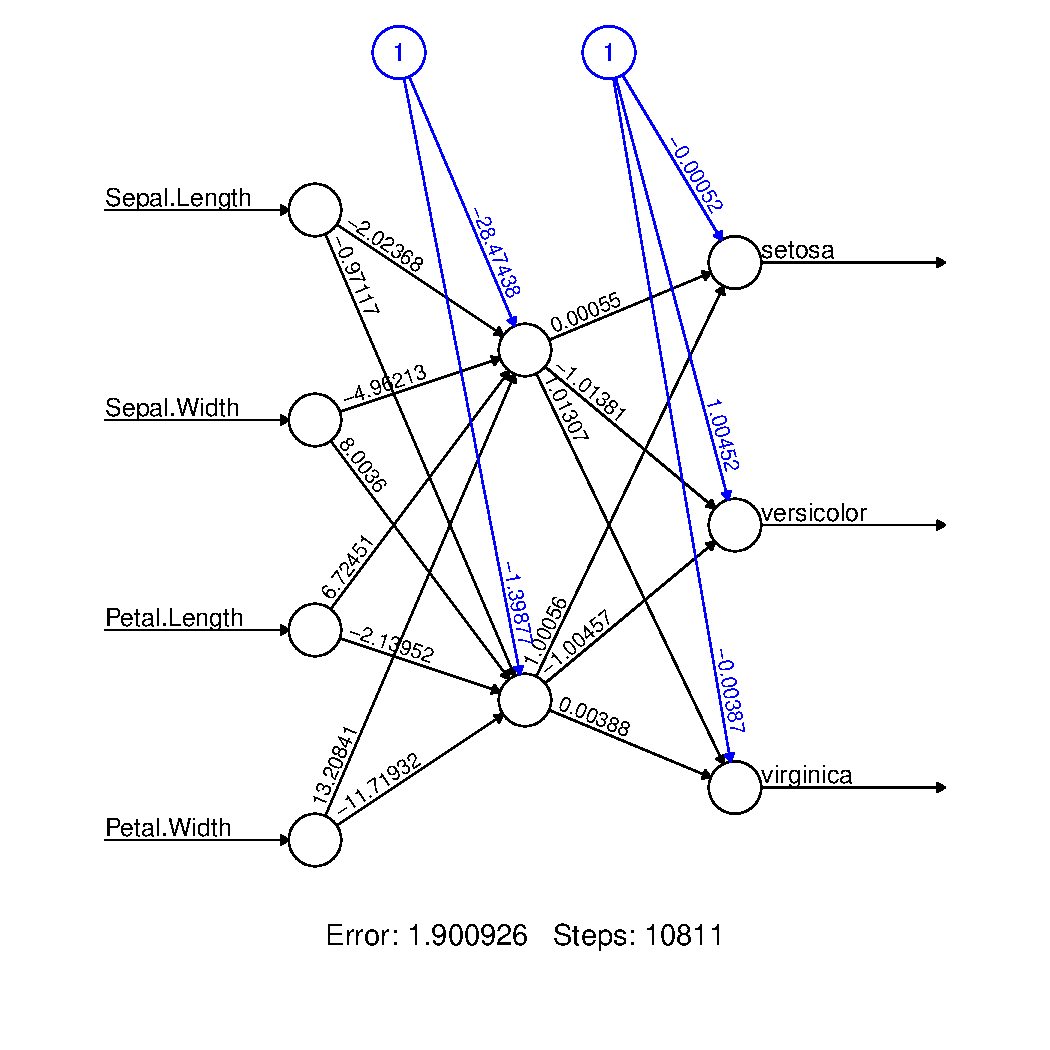
\includegraphics[width=4cm]{../../Graphs/NN_Iris.pdf}
\end{center}
Of course, the signs can help interpretation: $a_1^{(1)}=-2.0$ means the Sepal.Length increasing, increases $Z_1$. We also see that an increase in $Z_1$ increases "setosa" value and decreases "versicolor". 
\end{frame}
%%%%%%%%%%%%%%%%%%%%%%%%%%%%%
\begin{frame}
\frametitle{NN: interpretation}
Therefore, combination of signs can be used to try to interpret the effect of features on the output. However, neural network are not designed for this:
\begin{itemize}
\item Coefficients may vary a lot with the algorithm (for similar predictions)
\item Switch in the arrow/nodes are possible (e.g. change the signs above and the prediction will be the same)
\item Lots of layers/features makes this analysis intractable. 
\end{itemize}
\end{frame}
%%%%%%%%%%%%%%%%%%%%%%%%%%%%%
%\begin{frame}
%\frametitle{NN: generalization}
%A neural network can be seen as a network of logistic regressions at each node. Indeed, the sigmo\"{\i}d function is nothing else than the logit function.\\ 
%\vspace{0.3cm}
%In theory, another model could be used or even several type of models. Hence, for example, one can use Naive Bayes for all the nodes in a layer, logistic regression on the next layer, etc.\\
%\vspace{0.3cm}
%Therefore, a whole system of learning can be built through a neural network, adapting it closely to the data and the task.
%\end{frame}
%%%%%%%%%%%%%%%%%%%%%%%%%%%%%
\end{document} 
%%%%%%%%%%%%%%%%%%%%%%%%%%%%%
%%%%%%%%%%%%%%%%%%%%%%%%%%%%%
%%%%%%%%%%%%%%%%%%%%%%%%%%%%%
%%%%%%%%%%%%%%%%%%%%%%%%%%%%%
%%%%%%%%%%%%%%%%%%%%%%%%%%%%%
\begin{frame}
\frametitle{NN: deep learning}
For sure one of the most fashionable term in data science nowadays, if not the most. {\bf Deep Learning} is a sub-field\footnote{With so many applications that it is now a domain in itself.} of Machine Learning. One of its characteristics is that it uses very large (i.e. deep) neural networks to learn from the data. \\
\vspace{0.2cm}
In ML, one takes the features and feeds the model with them to predict an outcome. The features needs to be created and/or defined first. In some applications it is easy or even desirable. In others, the features are not so clear. Think about unstructured data like videos or texts.\\
\vspace{0.2cm}
The idea behind deep learning is to build a very large NN that will create the features from unstructured data in addition to building predictions. 
\end{frame}
%%%%%%%%%%%%%%%%%%%%%%%%%%%%%
https://www.r-bloggers.com/fitting-a-neural-network-in-r-neuralnet-package/
https://www.r-bloggers.com/multilabel-classification-with-neuralnet-package/
